\documentclass{article}

\usepackage{amsmath}
\usepackage{amsfonts} % For math fonts.
\usepackage{amssymb} % For other math symbols not covered by amsmath.
\usepackage[pdftex]{graphicx} % For pictures, use \includegraphics[scale=decimal]{pic.png}; must be a .png file type.
\usepackage{multicol}
\usepackage{textcomp}
\usepackage[colorlinks = true, urlcolor = blue]{hyperref}
\usepackage{enumitem}
\usepackage{graphbox} 
\usepackage{subfig}
\usepackage{multicol}
\usepackage{nopageno}


\usepackage{tikz}
\usetikzlibrary{positioning, calc}
\usetikzlibrary{shapes.geometric,angles,quotes}
\usepackage{tikz-3dplot}


%page formatting
\usepackage{fullpage}
\setlength{\parindent}{0pt}


\newcommand{\tab}{\hspace*{0.25in}}
\newcommand{\csq}[1]{\reflectbox{''}#1''}  %This produces CS style quotes.
\newcommand{\csqt}[1]{\text{\reflectbox{''}#1''}}  %This produces CS style quotes as text.


\usepackage{listings}
\lstset
{ %Formatting for code in appendix
    language=Python,
    basicstyle=\footnotesize,
    numbers=left,
    stepnumber=1,
    showstringspaces=false,
    tabsize=2,
    breaklines=true,
    breakatwhitespace=false,
}


\begin{document}



%split_point

%\end{document}
Matt Priem \hfill Expresions quiz\\
section 1\\
\begin{enumerate}
	\item 
		Write a program that calculates then outputs the volume of a right square pyramid.  
		The user should be able to pick $b$ (the base edge) and $h$ (the height).\\
		%Make sure to use the value of pi from the math module.\\
		Hint: $V = \dfrac{b^2 h}{3}$
		
		\vspace*{-4em}
		\begin{flushright}
		\tdplotsetmaincoords{70}{-20}
		\begin{tikzpicture}[tdplot_main_coords,line cap=butt,line join=bevel]
			\pgfmathsetmacro{\B}{4}
			\pgfmathsetmacro{\H}{4}
			\draw[thick] (-\B/2,-\B/2,0) -- (\B/2,-\B/2,0) -- (\B/2,\B/2,0) -- (-\B/2,\B/2,0)
				 -- cycle;
			\draw[thick] (\B/2,\B/2,0) -- (0,0,\H)
			node[above,font=\large\bfseries]{};
			\draw[dashed] (0,0,0) -- (0,0,\H) coordinate[midway](aux1);
			\draw[] (0,0,0.3) -- (0.3,0,0.3) -- (0.3,0,0);
			%\draw[dashed,blue] (-\B/2,0,0) -- (0,0,\H) coordinate[pos=0.3](aux2);
			%\draw[blue] ({-\B/2+0.15*(\H/\B)},0,0.3) -- ({-\B/2+0.15*(\H/\B)},-0.3,0.3) 
				%-- (-\B/2,-0.3,0);
			\coordinate (aux3) at (0.3,-2,0);
			\draw[thick] (-\B/2,-\B/2,0) -- (0,0,\H) -- (\B/2,-\B/2,0) -- cycle;
			\draw[thick] (-\B/2,-\B/2,0) -- (0,0,\H) -- (-\B/2,\B/2,0) -- cycle;
			\begin{scope}[tdplot_screen_coords]
				\draw (aux1) -- ++ (2,0.1) node[right,font=\itshape] {Height: h};
				%\draw (aux2) -- ++ (-1.5,0.3) node[left,font=\itshape] {Slant Height};
				\draw (aux3) -- ++ (2,-0.2) node[below right,font=\itshape] {Base edge: b};
			\end{scope}
		\end{tikzpicture}
		\end{flushright}


	\item
		%https://edabit.com/challenge/QzXtDnSZL6y4ZcEvT
		A farmer is asking you to tell him how many legs can be counted among all his animals. 
		The farmer breeds three species:
		\begin{itemize}
			\item chickens, which have \textbf{2} legs
			\item cows, which have \textbf{4} legs
			\item pigs, which have \textbf{4} legs
		\end{itemize}
		Write a program that asks the farmer how many of each animal he has, and then outputs the
		total number of legs.  		
		For example, \\ \ \hfill
		\includegraphics[height = 0.6in]{./imgs/animalLegs_ex1.PNG} \hfill
		\includegraphics[height = 0.6in]{./imgs/animalLegs_ex2.PNG} \hfill \
	
	
	
	

	\item 
		Write a program that calculates then outputs the area of a trapezoid.  
		The user should be able to pick both bases and the height (that is: $a$, $b$, and $h$).\\
		Hint: $A = \dfrac{a+b}{2}h$
		
		\vspace*{-3em}
		\begin{flushright}
		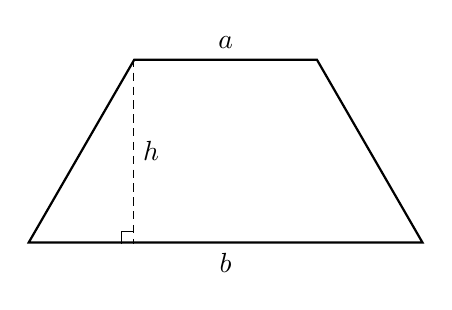
\begin{tikzpicture}
			\node (a) [trapezium, trapezium angle=60, minimum width=50mm, draw, thick, label=above:$a$,
				label=below:$b$] {};
			\draw [densely dashed] (a.north west) coordinate (a nw) -- (a nw |- a.south) node 
				[midway,right] {$h$};
			\draw (a nw |- a.south) ++(0,1.5mm) -| ++(-1.5mm,-1.5mm);
			\coordinate (a blc) at (a.bottom left corner);
			\coordinate (a brc) at (a.bottom right corner);
		\end{tikzpicture}
		\end{flushright}



\end{enumerate}
\pagebreak
Bart Simpson \hfill Expresions quiz\\
section 1\\
\begin{enumerate}
	\item 
		Write a program that calculates then outputs the area of a trapezoid.  
		The user should be able to pick both bases and the height (that is: $a$, $b$, and $h$).\\
		Hint: $A = \dfrac{a+b}{2}h$
		
		\vspace*{-3em}
		\begin{flushright}
		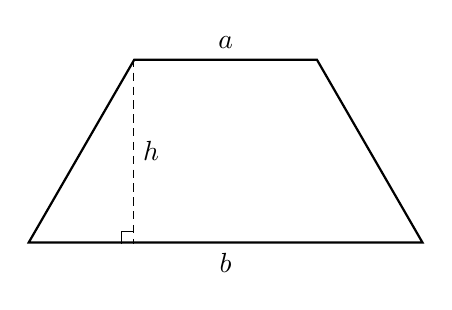
\begin{tikzpicture}
			\node (a) [trapezium, trapezium angle=60, minimum width=50mm, draw, thick, label=above:$a$,
				label=below:$b$] {};
			\draw [densely dashed] (a.north west) coordinate (a nw) -- (a nw |- a.south) node 
				[midway,right] {$h$};
			\draw (a nw |- a.south) ++(0,1.5mm) -| ++(-1.5mm,-1.5mm);
			\coordinate (a blc) at (a.bottom left corner);
			\coordinate (a brc) at (a.bottom right corner);
		\end{tikzpicture}
		\end{flushright}



	\item 
		You are counting points for a basketball game. Ask the user the amount of 3-pointers scored 
		and the amount 2-pointers scored, find the final points for the team and output the value.\\
		For example, if a team scored 5 2-pointers and 7 3-pointers, then their score would be 31.\\
		If a team scored 6 2-pointers and 5 3-pointers, then their score would be 27.
	
	
	\item
		Write a program that calculates and then outputs the volume of a sphere.  
		The user should be able to pick the radius.
		Use the value of $\pi$ from the math module in your calculation.\\	
		Hint: $V = \dfrac{4}{3}\pi r^3 $
	
		\begin{flushright}
			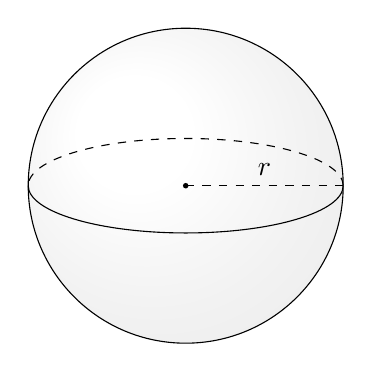
\begin{tikzpicture}
			\shade[ball color = white, opacity = 0.1] (0,0) circle (2cm);
			\draw (0,0) circle (2cm);
			\draw (-2,0) arc (180:360:2 and 0.6);
			\draw[dashed] (2,0) arc (0:180:2 and 0.6);
			\fill[fill=black] (0,0) circle (1pt);
			\draw[dashed] (0,0 ) -- node[above]{$r$} (2,0);
			\end{tikzpicture}
		\end{flushright}


\end{enumerate}
\pagebreak
Lone Star \hfill Expresions quiz\\
section 2\\
\begin{enumerate}
	\item
		Write a program that calculates the volume of a cylinder.  The user should be able to pick
		the height and radius.  Use the value of $\pi$ from the math module in your calculation.\\
		\tab Hint: $V = \pi r^2 h$\\

		\vspace*{-2em}
		\begin{flushright}
		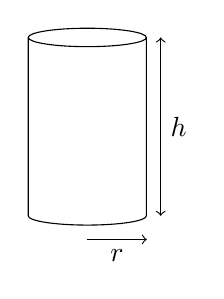
\begin{tikzpicture}
			\node (a) [cylinder, shape border rotate=90, draw, 
				minimum height=25mm, minimum width=15mm] {};
			\draw [<->] ([xshift=5pt]a.before bottom) -- ([xshift=5pt]a.after top)
				 node [midway, right] {$h$};
			\draw [->] ([yshift=-5pt]a.bottom) -- ([yshift=-5pt]a.bottom -| a.before bottom)
				node [midway, below] {$r$};
		\end{tikzpicture}
		\end{flushright}


	\item
		Write a program that calculates and then outputs the volume of a sphere.  
		The user should be able to pick the radius.
		Use the value of $\pi$ from the math module in your calculation.\\	
		Hint: $V = \dfrac{4}{3}\pi r^3 $
	
		\begin{flushright}
			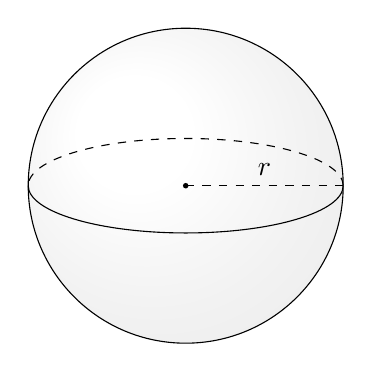
\begin{tikzpicture}
			\shade[ball color = white, opacity = 0.1] (0,0) circle (2cm);
			\draw (0,0) circle (2cm);
			\draw (-2,0) arc (180:360:2 and 0.6);
			\draw[dashed] (2,0) arc (0:180:2 and 0.6);
			\fill[fill=black] (0,0) circle (1pt);
			\draw[dashed] (0,0 ) -- node[above]{$r$} (2,0);
			\end{tikzpicture}
		\end{flushright}


	\item 
		Write a program that calculates then outputs the volume of a right square pyramid.  
		The user should be able to pick $b$ (the base edge) and $h$ (the height).\\
		%Make sure to use the value of pi from the math module.\\
		Hint: $V = \dfrac{b^2 h}{3}$
		
		\vspace*{-4em}
		\begin{flushright}
		\tdplotsetmaincoords{70}{-20}
		\begin{tikzpicture}[tdplot_main_coords,line cap=butt,line join=bevel]
			\pgfmathsetmacro{\B}{4}
			\pgfmathsetmacro{\H}{4}
			\draw[thick] (-\B/2,-\B/2,0) -- (\B/2,-\B/2,0) -- (\B/2,\B/2,0) -- (-\B/2,\B/2,0)
				 -- cycle;
			\draw[thick] (\B/2,\B/2,0) -- (0,0,\H)
			node[above,font=\large\bfseries]{};
			\draw[dashed] (0,0,0) -- (0,0,\H) coordinate[midway](aux1);
			\draw[] (0,0,0.3) -- (0.3,0,0.3) -- (0.3,0,0);
			%\draw[dashed,blue] (-\B/2,0,0) -- (0,0,\H) coordinate[pos=0.3](aux2);
			%\draw[blue] ({-\B/2+0.15*(\H/\B)},0,0.3) -- ({-\B/2+0.15*(\H/\B)},-0.3,0.3) 
				%-- (-\B/2,-0.3,0);
			\coordinate (aux3) at (0.3,-2,0);
			\draw[thick] (-\B/2,-\B/2,0) -- (0,0,\H) -- (\B/2,-\B/2,0) -- cycle;
			\draw[thick] (-\B/2,-\B/2,0) -- (0,0,\H) -- (-\B/2,\B/2,0) -- cycle;
			\begin{scope}[tdplot_screen_coords]
				\draw (aux1) -- ++ (2,0.1) node[right,font=\itshape] {Height: h};
				%\draw (aux2) -- ++ (-1.5,0.3) node[left,font=\itshape] {Slant Height};
				\draw (aux3) -- ++ (2,-0.2) node[below right,font=\itshape] {Base edge: b};
			\end{scope}
		\end{tikzpicture}
		\end{flushright}


\end{enumerate}
\pagebreak
Dot Matrix \hfill Expresions quiz\\
section 3\\
\begin{enumerate}
	\item
		Write a program that calculates and then outputs the volume of a sphere.  
		The user should be able to pick the radius.
		Use the value of $\pi$ from the math module in your calculation.\\	
		Hint: $V = \dfrac{4}{3}\pi r^3 $
	
		\begin{flushright}
			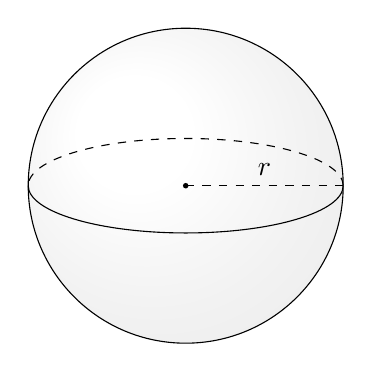
\begin{tikzpicture}
			\shade[ball color = white, opacity = 0.1] (0,0) circle (2cm);
			\draw (0,0) circle (2cm);
			\draw (-2,0) arc (180:360:2 and 0.6);
			\draw[dashed] (2,0) arc (0:180:2 and 0.6);
			\fill[fill=black] (0,0) circle (1pt);
			\draw[dashed] (0,0 ) -- node[above]{$r$} (2,0);
			\end{tikzpicture}
		\end{flushright}


	\item 
		Write a program that calculates then outputs the volume of a cone.  \\
		The user should be able to pick $r$ (the radius) and $h$ (the height).\\
		Use the value of $\pi$ from the math module in your calculation.\\	
		Hint: $V = \pi \cdot \dfrac{r^2 h}{3}$ \vspace*{-5em}
		\begin{flushright}
		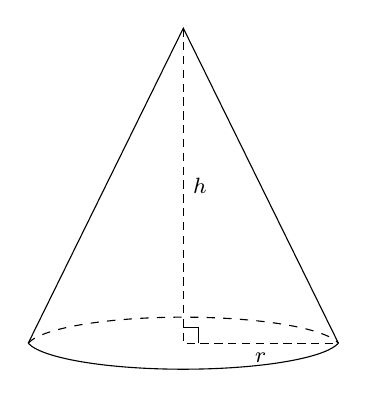
\begin{tikzpicture}
			\draw[dashed] (0,0) arc (170:10:2cm and 0.4cm)coordinate[pos=0] (a);
			\draw (0,0) arc (-170:-10:2cm and 0.4cm)coordinate (b);
			\draw[densely dashed] ([yshift=4cm]$(a)!0.5!(b)$) 
				-- node[right,font=\footnotesize]{$h$}coordinate[pos=0.95] (aa)($(a)!0.5!(b)$)
				-- node[below,font=\footnotesize] {$r$}coordinate[pos=0.1] (bb) (b);
    		\draw (aa) -| (bb);
    		\draw (a) -- ([yshift=4cm]$(a)!0.5!(b)$) -- (b);
  		\end{tikzpicture}
	\end{flushright}


	\item
		%https://edabit.com/challenge/QzXtDnSZL6y4ZcEvT
		A farmer is asking you to tell him how many legs can be counted among all his animals. 
		The farmer breeds three species:
		\begin{itemize}
			\item chickens, which have \textbf{2} legs
			\item cows, which have \textbf{4} legs
			\item pigs, which have \textbf{4} legs
		\end{itemize}
		Write a program that asks the farmer how many of each animal he has, and then outputs the
		total number of legs.  		
		For example, \\ \ \hfill
		\includegraphics[height = 0.6in]{./imgs/animalLegs_ex1.PNG} \hfill
		\includegraphics[height = 0.6in]{./imgs/animalLegs_ex2.PNG} \hfill \
	
	
	
	

\end{enumerate}
\pagebreak
Alfred Yankovic \hfill Expresions quiz\\
section 2\\
\begin{enumerate}
	\item 
		Write a program that calculates then outputs the area of a trapezoid.  
		The user should be able to pick both bases and the height (that is: $a$, $b$, and $h$).\\
		Hint: $A = \dfrac{a+b}{2}h$
		
		\vspace*{-3em}
		\begin{flushright}
		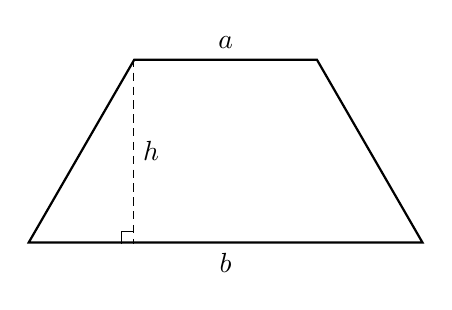
\begin{tikzpicture}
			\node (a) [trapezium, trapezium angle=60, minimum width=50mm, draw, thick, label=above:$a$,
				label=below:$b$] {};
			\draw [densely dashed] (a.north west) coordinate (a nw) -- (a nw |- a.south) node 
				[midway,right] {$h$};
			\draw (a nw |- a.south) ++(0,1.5mm) -| ++(-1.5mm,-1.5mm);
			\coordinate (a blc) at (a.bottom left corner);
			\coordinate (a brc) at (a.bottom right corner);
		\end{tikzpicture}
		\end{flushright}



	\item 
		You are counting points for a basketball game. Ask the user the amount of 3-pointers scored 
		and the amount 2-pointers scored, find the final points for the team and output the value.\\
		For example, if a team scored 5 2-pointers and 7 3-pointers, then their score would be 31.\\
		If a team scored 6 2-pointers and 5 3-pointers, then their score would be 27.
	
	
	\item 
		Write a program that calculates then outputs the volume of a right square pyramid.  
		The user should be able to pick $b$ (the base edge) and $h$ (the height).\\
		%Make sure to use the value of pi from the math module.\\
		Hint: $V = \dfrac{b^2 h}{3}$
		
		\vspace*{-4em}
		\begin{flushright}
		\tdplotsetmaincoords{70}{-20}
		\begin{tikzpicture}[tdplot_main_coords,line cap=butt,line join=bevel]
			\pgfmathsetmacro{\B}{4}
			\pgfmathsetmacro{\H}{4}
			\draw[thick] (-\B/2,-\B/2,0) -- (\B/2,-\B/2,0) -- (\B/2,\B/2,0) -- (-\B/2,\B/2,0)
				 -- cycle;
			\draw[thick] (\B/2,\B/2,0) -- (0,0,\H)
			node[above,font=\large\bfseries]{};
			\draw[dashed] (0,0,0) -- (0,0,\H) coordinate[midway](aux1);
			\draw[] (0,0,0.3) -- (0.3,0,0.3) -- (0.3,0,0);
			%\draw[dashed,blue] (-\B/2,0,0) -- (0,0,\H) coordinate[pos=0.3](aux2);
			%\draw[blue] ({-\B/2+0.15*(\H/\B)},0,0.3) -- ({-\B/2+0.15*(\H/\B)},-0.3,0.3) 
				%-- (-\B/2,-0.3,0);
			\coordinate (aux3) at (0.3,-2,0);
			\draw[thick] (-\B/2,-\B/2,0) -- (0,0,\H) -- (\B/2,-\B/2,0) -- cycle;
			\draw[thick] (-\B/2,-\B/2,0) -- (0,0,\H) -- (-\B/2,\B/2,0) -- cycle;
			\begin{scope}[tdplot_screen_coords]
				\draw (aux1) -- ++ (2,0.1) node[right,font=\itshape] {Height: h};
				%\draw (aux2) -- ++ (-1.5,0.3) node[left,font=\itshape] {Slant Height};
				\draw (aux3) -- ++ (2,-0.2) node[below right,font=\itshape] {Base edge: b};
			\end{scope}
		\end{tikzpicture}
		\end{flushright}


\end{enumerate}
\pagebreak
\end{document}